\documentclass{beamer}
\usetheme{Madrid}

\title[Wobbling Motion in Odd-Mass Nuclei] % (optional, only for long titles)
{Wobbling Motion in odd-mass nuclei}
\author[R. Poenaru] % (optional, for multiple authors)
{Robert Poenaru\inst{1,2}}
\institute[DFT @ IFIN-HH] % (optional)
{
  \inst{1}%
  Department of Theoretical Physics\newline
  IFIN-HH
  \and
  \inst{2}%
  Faculty of Physics\newline
  University of Bucharest
}
\date[\today] % (optional)
{Bucharest University Faculty of Physics 2021 Meeting}
\subject{Nuclear Physics}

\begin{document}
\maketitle
\begin{frame}
\frametitle{Table of Contents}
\tableofcontents
\section{Introduction}
\end{frame}
\begin{frame}
    \frametitle{Example of columns 1}
    \begin{columns}[c] % the "c" option specifies center vertical alignment
    \column{.45\textwidth} % column designated by a command
     Contents of the first column
    \column{.45\textwidth}
     Contents split \newline into two lines
    \end{columns}
\end{frame}


\begin{frame}{Nuclear Wobbling Motion}
      \begin{figure}
          \centering
          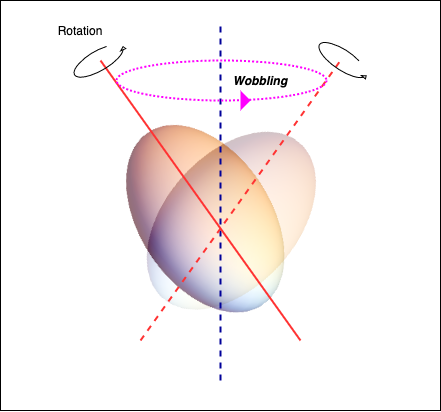
\includegraphics[scale=0.45]{figs/wobbling_drawing.png}
          \caption{Schematic representation for the nuclear wobbling motion.}
          \label{wobbling_picture}
      \end{figure}
\end{frame}
\section{Triaxial nuclei}

  \begin{frame}
    \frametitle{This is the second slide}
  \end{frame}

\section{Results}  

  \begin{frame}
    \frametitle{This is the second slide}
  \end{frame}

\section{Future Plans}

  \begin{frame}
    \frametitle{This is the second slide}
  \end{frame}

\section{Conclusions}

  \begin{frame}
    \frametitle{This is the second slide}
  \end{frame}

\end{document}